\begin{figure*}[tb]
    \centering
    \subfloat[\label{typical}Typical Experiment Lifecycle]{
        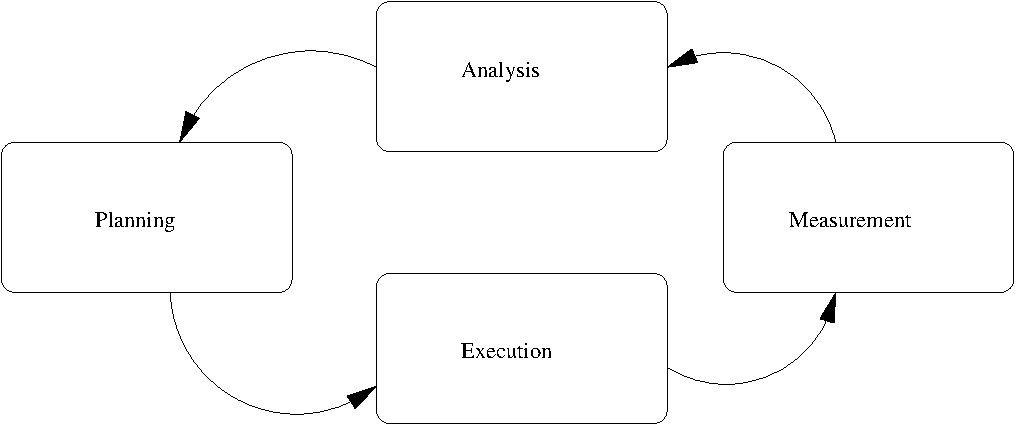
\includegraphics[width=0.4\textwidth]{figs/planning.pdf}
    }
    \hspace{0.5in}
    \subfloat[\label{lem-plan}\name\ Augmented Experiment Lifecycle]{
        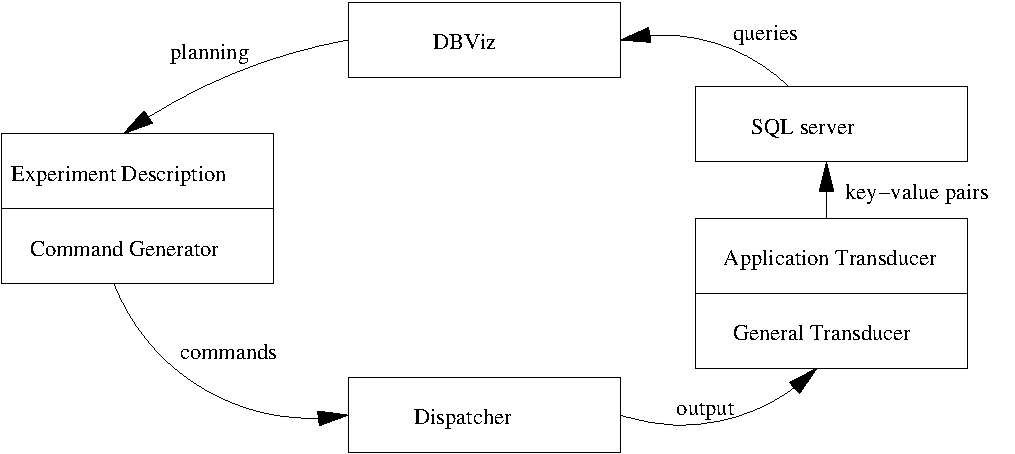
\includegraphics[width=0.4\textwidth]{figs/arch.pdf}
    }
    \mycaption{fig-plan}{Experiment Lifecycle.}{
The figure on the left depicts a typical experiment lifecycle progressing
through planning, execution, measurement, and analysis.  A user devises an
experiment to study the effect of some number of independent variables,
executes and measures each \sub, analyzes the results, and, depending on that
analysis, can then revise the experiment and repeat the cycle.  The figure on
the right shows the workflow within \name.  The user describes their parameter
space to the \cg\ and specifies a path to an optional application transducer to
capture application specific \kv\ pairs.  \name\ adds a path to a general
transducer to capture \kv\ pairs common to all experiments.  The generated
commands and their transducer(s) are then passed to the \dispatcher\ which
either submits the commands to a scheduling system or runs them synchronously
in the foreground.  As the commands run, \kv\ pairs are captured by the
transducer(s) and inserted into a SQL server from which they can then be
queried to visualize and analyze the results.  Depending on this analysis the
user can then modify their parameter space and repeat the cycle.
}
\end{figure*}
